\begin{tikzpicture}[
	scale=0.78, every node/.style={transform shape},
	actor/.style={rectangle, rounded corners, draw=black, fill=gray!15, minimum width=3.4cm, minimum height=1.1cm, font=\bfseries, align=center, inner sep=4pt},
	stepbox/.style={rectangle, rounded corners, draw=#1, fill=#1!8, line width=0.8pt, font=\small, align=center, inner sep=6pt},
	msgarrow/.style={->, >=stealth, line width=1pt, #1},
	badge/.style={circle, fill=#1, text=white, font=\bfseries\footnotesize, inner sep=2pt}
]
	% Spaltenkoordinaten
	\def\colA{0}     % Alice
	\def\colCA{5.5}  % CA
	\def\colB{11}    % Bob

	% --- AKTEURE (Kopfzeile) ---
	\node[actor] (alice) at (\colA, 0) {Alice\\{\footnotesize (Absenderin)}\\[2pt]{\scriptsize öff.: $(e_A, n_A)$,\; priv.: $d_A$}};
	\node[actor, fill=DarkOrchid!15, draw=DarkOrchid] (ca) at (\colCA, 0) {\textcolor{DarkOrchid}{\faCertificate{}} CA\\{\footnotesize (Zertifizierungsstelle)}\\[2pt]{\scriptsize öff.: $(e_{\text{CA}}, n_{\text{CA}})$,\; priv.: $d_{\text{CA}}$}};
	\node[actor] (bob) at (\colB, 0) {Bob\\{\footnotesize (Empfänger)}\\[2pt]{\scriptsize vorinstalliert: $(e_{\text{CA}}, n_{\text{CA}})$}};

	% Vertikale Hilfslinien
	\draw[dashed, gray!40] (alice.south) -- (\colA, -13.8);
	\draw[dashed, gray!40] (ca.south) -- (\colCA, -5.8);
	\draw[dashed, gray!40] (bob.south) -- (\colB, -13.8);

	% --- PHASE 1: ZERTIFIZIERUNG (VORAB) ---
	\node[font=\footnotesize\bfseries\color{DarkOrchid!80!black}, fill=white, inner sep=2pt] at (\colCA, -1.1) {Phase 1: Zertifikatserstellung (einmalig vorab)};

	% Pfeil 1: Alice -> CA (Schlüsselregistrierung)
	\node[badge=RoyalBlue] (b1) at (\colA+0.6, -2.0) {1};
	\draw[msgarrow=RoyalBlue] (b1.east) -- (\colCA-0.3, -2.0)
		node[midway, above=2pt, font=\footnotesize] {Antrag mit Daten $z = (\text{\enquote{Alice}}, e_A, n_A)$};

	% CA signiert
	\node[stepbox=DarkOrchid] (ca_sign) at (\colCA, -3.4) {
		\textbf{CA prüft Identität \& signiert $z$:}\\
		$\text{Cert}_A := z^{d_{\text{CA}}} \bmod n_{\text{CA}}$
	};

	% Pfeil 2: CA -> Alice (Zertifikatsausgabe)
	\node[badge=DarkOrchid] (b2) at (\colCA-0.6, -4.8) {2};
	\draw[msgarrow=DarkOrchid] (b2.west) -- (\colA+0.3, -4.8)
		node[midway, above=2pt, font=\footnotesize] {Ausgabe: Zertifikat $(z, \text{Cert}_A)$};

	% --- PHASE 2: VERSAND DER SIGNIERTEN NACHRICHT ---
	\node[font=\footnotesize\bfseries\color{RoyalBlue!80!black}, fill=white, inner sep=2pt] at (5.5, -6.0) {Phase 2: Signieren \& Übertragen};

	% Alice signiert
	\node[stepbox=RoyalBlue] (alice_sign) at (\colA, -7.3) {
		\textbf{Alice signiert Vertrag $m$:}\\
		$s := m^{d_A} \bmod n_A$
	};

	% Pfeil 3: Alice -> Bob
	\node[badge=black] (b3) at (\colA+1.8, -9.0) {3};
	\draw[msgarrow=black] (b3.east) -- (\colB-1.8, -9.0)
		node[midway, above=3pt, font=\footnotesize, align=center] {Vertrag $m$ \quad+\quad Signatur $s$ \quad+\quad Zertifikat $(z, \text{Cert}_A)$};

	% --- PHASE 3: ZWEISTUFIGE VERIFIKATION BEI BOB ---
	\node[font=\footnotesize\bfseries\color{ForestGreen!80!black}, fill=white, inner sep=2pt] at (\colB, -10.3) {Phase 3: Verifikation bei Bob};

	% Bob Verifikation
	\node[stepbox=ForestGreen] (bob_verify) at (\colB, -12.1) {
		\textbf{Schritt A: Zertifikat mit $(e_{\text{CA}}, n_{\text{CA}})$ prüfen}\\
		$z' := (\text{Cert}_A)^{e_{\text{CA}}} \bmod n_{\text{CA}}$\\
		$\rightarrow \text{Gilt } z' = z\text{?} \implies (e_A, n_A)\text{ ist echt!}$\\[4pt]
		\textbf{Schritt B: Signatur mit $(e_A, n_A)$ prüfen}\\
		$m' := s^{e_A} \bmod n_A$\\
		$\rightarrow \text{Gilt } m' = m\text{?} \implies \text{Vertrag ist echt!} \textcolor{ForestGreen}{\mathbf{\checkmark}}$
	};
\end{tikzpicture}
